
\chapter{Design of antimicrobial peptides}\label{chapter:amps}

\section{Introduction}
    In the previous chapter, I introduced grammars as a generalized
    method for modeling motifs in sequences of characters.  In
    addition, I presented a detailed look at the Teiresias motif
    discovery tool.  In this, the second chapter of my thesis, I
    show how Teiresias can be used to derive sets of regular
    grammars describing a particular class of protein sequences ---
    antimicrobial peptides.  In what follows, I present a general
    background on antimicrobial peptides and then provide a
    rationale for why these peptides are particularly well--suited
    for being modeled using regular grammars.  I detail the
    construction of an annotation tool for finding new antimicrobial
    peptides and validating the general hypothesis that regular
    grammars can be used as a sensitive and specific indicator of
    antimicrobial function in peptide sequences.  Next, I describe
    the preliminary design of synthetic antimicrobial peptides using
    an evolutionary approach, which, although ultimately inconclusive, provided
    motivation for a more focused design.  The final section of this
    chapter describes a more focused design approach, detailing the
    successful construction of numerous novel peptides with strong
    antimicrobial activity against a wide spectrum of bacteria.

    The research described in this chapter is drawn
    largely from a publication that is in preparation
    in collaboration with Christopher Loose, Isidore
    Rigoutsos, and Gregory Stephanopoulos.  (Some
    experimental work in Section~\vref{section:preliminary}
    was also performed by Gyoo Yeol Jung.)  Throughout this
    chapter, the use of the pronoun ``we'' refers to this
    group of authors.

\section{Motivation}
    Antimicrobial peptides are small
    proteins that attack and kill microbes.
    These peptides are effectors of the
    innate immune system: the phylogenetically
    ancient first line of defense against pathogen
    assault~\cite{rolff2003invertebrate,kimbrell2001evolution}.
    Antimicrobial peptides are ubiquitous
    amongst multicellular eukaryotes and
    found in diverse contexts including frog
    skin~\cite{simmaco1999antimicrobial}, scorpion
    venom~\cite{moerman2002antibacterial}, and human
    sweat~\cite{schittek2001dermcidin}.

    There is a growing interest in antimicrobial
    peptides, due largely to the proliferation
    of multi--drug resistant pathogen
    strains~\cite{cassell2001development}.  These
    strains are resistant to one or more common
    antibiotics such as penicillin, tetracylin,
    or vanocomycin.  In the United States alone,
    the cost of treating and preventing infections by
    these pathogens is estimated to be many billions of
    dollars annually~\cite{harrison1998antimicrobial}.
    In the arms race against microbes,
    mankind is losing --- only a single new
    class of antibiotics was developed in the
    past 30 years~\cite{normark2002evolution,
    walsh2000molecular}.  However, there is mounting
    evidence that antimicrobial peptides are less
    likely to induce bacterial resistance and will make
    a strong contribution to our therapeutic arsenal
    ~\cite{zasloff2002antimicrobial,zasloff2002antimicrobialpeptides,ge1999invitro}.

    Human antimicrobial peptides, such as
    the defensins and cathelicidins, help to
    maintain a passive defense against pathogens
    in the environment.  A malfunction of these
    peptides leads to severely immunocompromised
    phenotypes.  For example, a deficiency of the
    LL-37 cathelicidin leads to morbus Kostmann,
    a congenital neutropenia characterized
    by recurrent bacterial infection and short
    life--expectancy~\cite{putsep2002deficiency,bowman2003antibacterial}.
    In addition, the pathogenesis of cystic fibrosis
    (CF) is indirectly caused by antimicrobial peptide
    impairment~\cite{ganz2003defensins}.  CF patients
    have a defective Cl$^-$ ion channel in the
    pulmonary airway epithelia that causes unusually
    high salt concentrations.  The salt disrupts the
    function of the epithelial defensins, leading
    to chronic infections and ensuing respiratory
    failure~\cite{smith1996cystic,zasloff2002antimicrobial}.
    More severe phenotypes have been produced in
    loss--of--function animal models.  For example,
    Wilson \emph{et. al.}~\cite{wilson1999regulation}
    showed that mice with depressed defensin
    activity required a 10--fold lower dose
    of the \emph{S. typhimurium} pathogen
    to produce a fatality.  In contrast,
    gain--of--function mice expressing human
    enteric defensin HBD--5 have a markedly
    increased resistance to \emph{S. typhimurium}
    assault~\cite{salzman2003protection}.

    In addition to their more publicized
    antibiotic capabilities, antimicrobial peptides
    appear to be important in a variety of other
    diseases.  For example, the antimicrobial
    peptides of \emph{Anopheles gambiae},
    the malaria mosquito, are upregulated
    after malaria (\emph{Plasmodium berghei})
    infection~\cite{christophides2002immunity}
    and, in some cases, are capable
    of killing the ookinetes of the
    parasite~\cite{barillas2000mosquito,vizioli2001gambicin}.
    Antimicrobial peptides are also indicated in a
    resistance to the AIDS--causing virus, HIV\@.
    Long--term HIV nonprogressors display
    elevated levels of $\alpha$--defensins
    that inhibit the proliferation of the
    virus~\cite{zhang2002contribution}.
    Finally, a limited class of antimicrobial
    peptides may form the basis for novel cancer
    treatments~\cite{kim2003invitro,ellerby1999anticancer}.
    For example, the antimicrobial peptide
    tachyplesin can repress the growth of cancerous
    tumors both \emph{in vitro} and \emph{in
    vivo}~\cite{chen2001rgdtachyplesin}.

    The many disease--relevant behaviors of
    antimicrobial peptides are a result of their
    ability to broadly distinguish eukaryotic
    cells from pathogenic invaders.  There are two
    features that give the peptides this ability:
    a net positive charge and an amphipathic 3--D
    structure~\cite{giangaspero2001amphipathic,epand1999diversity}.
    These features endow the peptide with an
    affinity for negatively charged outer leaflet
    of the bacterial cytoplasmic membrane (see
    Figure~\vref{fig:peptideAction}).  This affinity
    leads to permeablization of the bacterial membrane,
    which is the basis for the bactericidal activity
    of antimicrobial peptides.  Although this mode
    of action is common to almost all antimicrobial
    peptides, there are many diverse primary sequences
    that can produce this behavior.  These sequences
    form a handful of conserved families, the most
    common of which are the $\alpha$--helical
    and $\beta$--sheet antimicrobial peptides
    ~\cite{tossi2000amphipathic}.

    \begin{figure}[phtb] \centering
    \includegraphics[width=0.70\textwidth]{Body/Images-chap2/attack2.png}
    \caption[Antimicrobial peptide action]{
        Antimicrobial peptide action.  In the
        figure above, amphipathic antimicrobial
        peptides with net positive charges are
        attracted via electrostatic forces to
        the negatively charged outer--leaflet
        of the microbial membrane (step
        1)~\cite{zasloff2002antimicrobial}.  This
        membrane is either the lipopolysaccharide
        layer or the peptidoglycan layer of
        gram--negative and gram--positive bacteria,
        respectively~\cite{epand1999diversity}.
        In addition, the $\beta$--1,3--glucan in
        fungal membranes and the phosphoglycan
        of certain parasites can give membrane
        characteristics that are exploited
        by certain classes of antimicrobial
        peptides.  The peptides cover and lyse
        the membrane via either a ``barrel
        stave'' or ``carpet'' mechanism (step
        2)~\cite{shai2002mode}.  Although some
        antimicrobial peptides are hemolytic,
        in general, they are not damaging to
        multicellular organisms because 1) the
        negatively charged phosphatydilserines
        of their outer leaflet are sequestered
        on the cytoplasmic side of the membrane,
        and 2) the membranes are stabilized by
        cholesterols~\cite{zasloff2002antimicrobial}.
    } \label{fig:peptideAction} \end{figure}


Figure~\vref{fig:aurein} shows the structure of aurein--1.2, an
archetypal alpha helical antimicrobial peptide from the Australian
Southern bell frog~\cite{wang2005correlation}.  Alpha helical AmPs
form the largest single family of AmPs.  They are particularly
common in amphibians because species such as frogs tend to inhabit
wet and warm ecological niches that are conducive to the
proliferation of bacteria.  (See Figure~\ref{fig:frogAmps} for a
phylogenetic tree of the more than 400 amphibian AmPs.)  Alpha
helical AmPs tend, in general, to have a amphipathic structure in
which positively charged residues are segregated on to a particular
side of the longitudinal axis of the helix.  Negatively charged or
neutral residues tend to be isolated on the opposite side from the
positively charged residues.  Evidence suggests that this
confirmation allows the peptide to position itself judiciously
relative to the bacterial membrane, facilitating entry of the
peptide into the membrane and, ultimately, membrane
disruption~\cite{zasloff2002antimicrobial}.

        \begin{figure}[ptb]
        A) Ball and stick
        \begin{center}
        \includegraphics[width=2.0in]{Body/Images-chap2/1vm5-balls.png}
        \end{center}

        \smallskip
        B) Ribbon
        \begin{center}
        \includegraphics[width=2.0in]{Body/Images-chap2/1vm5-ribbon.png}
        \end{center}

        \smallskip
        C) Peptide wheel view
        \begin{center}
        \includegraphics[angle=90,width=2.0in]{Body/Images-chap2/pepwheel.pdf}
        \end{center}
        \caption[The structure of aurein]{The structure of aurein--1.2~\cite{wang2005correlation}.
            Aureins constitute a large family of secreted proteins
            originally isolated from the skin of frogs.
            This particular structure was isolated from the
            Australian Southern bell frog.  The peptide conforms to
            the classic amphipathic alpha helical structure and has wide--spectrum antimicrobial activity.
            Part A) shows a ball--and--stick representation of the
            structure in which nitrogen atoms are colored blue and
            oxygen atoms are colored red.  Part B) shows the same
            structure using a cartoon representation that clearly
            shows the alpha helix.  Finally, part C) shows a helical
            wheel projection in which uncharged residues are boxed
            in order to highlight the segregation of charges on the
            helix.  Graphics created using PyMol (DeLano Scientific,
        San Carlos, CA, USA).
        }
        \label{fig:aurein}
        \end{figure}

        \begin{sidewaysfigure}[ptb]
        \begin{center}
        \includegraphics[angle=270,width=0.9\textwidth]{Body/Images-chap2/frog-amps.pdf}
        \end{center}
        \caption[A phylogenetic tree of amphibian antimicrobial peptides]{
            A phylogenetic tree of amphibian AmPs.  Because they
            tend to inhabit environments that are conducive to the
            growth of bacteria, amphibians are under evolutionary
            pressure to develop numerous and varied AmPs.  This tree
            shows the degree of sequence similarity for over 400
            AmPs isolated from amphibian sources.  As the figure
            shows, amphibians have many families of AmPs, some of
            which are only distantly related, including the aureins,
            bombinins, bombesins, and brevinins.
        }
        \label{fig:frogAmps}
        \end{sidewaysfigure}

    The characteristic membrane--attack of
    antimicrobial peptides is the primary
    rationalization of the peptides' propensity to
    not induce bacterial resistance to the same
    degree as small molecule pharmaceuticals.
    That is, because the peptides leverage a
    pervasive polygenic trait of bacteria, the
    structure of the cell wall, it is ``expensive''
    for the bacteria to evolve a resistance
    ~\cite{zasloff2002antimicrobial,zasloff2002antimicrobialpeptides}.
    For this reason, many companies are developing
    therapeutics based on antimicrobial
    peptides, many of which are in phase III
    FDA trials ~\cite{hancock2002clinical}.
    Even more encouraging, some peptides show
    strong \emph{in vitro} bactericidal activity
    against pathogen strains that have developed
    a resistance to multiple conventional
    antibiotics~\cite{ge1999invitro,tiozzo1998wide,strom2003pharmacophore}.

\section{A grammatical approach to annotating
AmPs}\label{section:annotation}
    Our preliminary studies of natural AmPs indicated that their
    amphipathic structure gives rise to a modularity among the different
    AmP amino acid sequences.  The repeated usage of sequence modules ---
    which may be a relic of evolutionary divergence and radiation ---
    is reminiscent of phrases in a natural language, such as English.
    For example, the grammar \texttt{Q.EAG.L.K..K} (the ``\texttt{.}'' is
    a ``wildcard'', which indicates that any amino acid will suffice at
    that position in the grammar) is present in over 90\% of cecropins,
    an AmP common in insects.  Based on this observation we modeled
    the AmP sequences as a formal language --- a set of sentences using
    characters from a fixed alphabet, in this case the alphabet of amino
    acid one--letter symbols~\cite{jurafsky2000speech}.

    We conjectured that the ``language of AmPs'' could be described
    by a set of regular grammars and that these grammars, in turn, could be used
    to annotate and design novel AmPs.  As discussed in
    Chapter~\ref{chapter:intro},
    regular grammars are, in
    essence, simple rules for describing the allowed arrangements of
    characters.  These grammars, such as the cecropin grammar mentioned
    previously, are commonly written as regular expressions and are
    widely used to describe patterns in nucleotide and amino acid
    sequences~\cite{searls2002language,hofmann1999prosite}.

    To find a set of grammars describing AmPs we used the
    Teiresias pattern discovery tool~\cite{rigoutsos1998combinatorial}
    (see Section~\vref{section:teiresias} to discover an
    exhaustive, maximal set of regular grammars in a collection of
    antimicrobial peptides assembled from a variety of sources.

    \subsection{Collecting a database of antimicrobial peptides}

    Our collection of known antimicrobial peptides was taken principally
    from two databases:
    the Antimicrobial Sequences
    Database (\amsdb) ~\cite{tossi2002antimicrobial} and
    \sptr ~\cite{bairoch2000swiss-prot}.
        The \amsdb~ contains
        about 750 antimicrobial peptides, all of which are
        a subset of \sptr .  Some of the entries in
        the \amsdb~ are sequence fragments that are derived
        from larger precursors via post--translational modification.
        We discarded these peptides unless the reported
        antimicrobial fragment comprised at least 80\% of the
        length of its parent sequence.  From the remaining
        entries, we selected all that were from eukaryotic organisms,
        including the complete length of the parent
        peptides in our database.



        
\begin{table}[!hbtp]
\centering
\caption{Common antimicrobial peptide families}\label{table:antimicrobialnames}
\begin{tabular}{cccc} \hline \hline
\small acaloleptin & 
\small achacin & 
\small adenoregulin & 
\small alpha--defensin \\ 
\small androctonin &
\small andropin & 
\small apidaecin & 
\small attacin \\
\small aurein & 
\small azurocidin & 
\small bactenecin & 
\small bactericidin \\ 
\small bactinecin & 
\small beta--defensin & 
\small bombinin & 
\small bombolitin \\
\small buforin & 
\small buthinin & 
\small caerin & 
\small caltrin \\
\small cathelin & 
\small cecropin & 
\small ceratotoxin & 
\small citropin \\ 
\small clavanin & 
\small coleoptericin & 
\small corticostatin & 
\small crabrolin \\ 
\small defensin & 
\small demidefensin & 
\small dermaseptin & 
\small dermcidin \\
\small diptericin & 
\small drosocin & 
\small drosomycin & 
\small enbocin \\
\small formaecin & 
\small gaegurin & 
\small gallinacin & 
\small gloverin \\ 
\small granulysin & 
\small hadrurin & 
\small heliomicin & 
\small hemiptericin \\ 
\small hemolin & 
\small hepcidin & 
\small histatin & 
\small holotricin \\
\small hymenoptaecin & 
\small hyphancin &
\small indolicidin & 
\small lebocin \\
\small macin & 
\small maculatin & 
\small maximin & 
\small metalnikowin \\ 
\small metchnikowin & 
\small misgurin & 
\small moricin & 
\small myticin \\
\small mytilin & 
\small mytimycin & 
\small nk--lysin & 
\small penaeidin \\ 
\small permatin & 
\small phormicin & 
\small phylloxin &
\small pleurocidin \\ 
\small polyphemusin & 
\small ponericin & 
\small protegrin & 
\small pseudin \\
\small pyrrhocoricin & 
\small ranalexin & 
\small ranatuerin & 
\small rhinocerosin \\ 
\small royalisin & 
\small rugosin & 
\small salmocidin & 
\small sapecin \\
\small sarcotoxin & 
\small sillucin & 
\small spingerin & 
\small styelin \\
\small tachycitin & 
\small tachyplesin & 
\small temporin & 
\small tenecin \\
\small termicin & 
\small thanatin & 
\small tricholongin & 
\small zeamatin \\ \hline \hline
\end{tabular}
\end{table}


        \sptr~ is a database of about 120 thousand heavily annotated
        sequences.  Included in the  annotations are keywords grouping
        proteins into functional categories.  For our initial database
        of antimicrobial peptides we extracted all the eukaryotic
        sequences matching
        the keywords ``antibiotic'', ``fungicidal'', or ``defensin''.
        These sequences were added to the peptides we collected
        from the ~\amsdb.

        Using the sequences that we extracted from \amsdb~ and \sptr,
        we made a list of
        common antimicrobial peptide names --- such as ``defensin'' or
        ``tenesin'' --- and collected sequences from \sptr~ matching these
        names.  From the name--matched sequences, we manually selected
        those eukaryotic sequences that had literature evidence of
        antimicrobial activity but were not explicitly
        labeled as such in \sptr.  These sequences, together with the
        sequences from \amsdb~ and the first set from \sptr, formed our initial database
        of antimicrobial peptides.  In the following section, we describe
        how these sequences were used, via a homology--based bootstrapping
        method, to find even more antimicrobial peptides within \sptr.

    \subsection{Finding more antimicrobial peptides}
        A minority of the antimicrobial peptides within \sptr, were not
        found using either the keyword or ``common--name'' searches.  To find
        these sequences we used two approaches in parallel.  First, we used
        a \Fasta~ sequence alignment based approach.  Second, we used a grammar matching--based
        approach with \Teiresias.  Both of these approaches are detailed below
        and summarized in Figure~\ref{fig:bootstrapping}.

        \begin{figure}[ptb]
        \centering
        \includegraphics{Body/Images-chap2/bootstrap.pdf}
        \caption[Schematic of the bootstrapping method.]{
            A schematic of the bootstrapping
            method used to collect
            antimicrobial sequences from \sptr
            .  On the left, using \Teiresias,
            we computed an 8/8/2 grammar set
            ($C_i^{8/2/2}$) from the initial
            set of sequences, $S_0$.  These
            grammars were masked from $S_0$
            to make $S_0\mid_{\textrm{m--}8/8/2}$,
            from which the 6/15/2 grammar set,
            $C_0\mid_{\textrm{m--}8/2/2}^{6/15/2}$,
            was found using \Teiresias~ again.
            The two grammar sets were combined
            and processed (see Appendix)
            to make $\phi'$.  This final
            grammar set was used to find more
            antimicrobial sequences in \sptr.
            On the right side of the schematic,
            sequences from $S_0$ were aligned
            against \sptr~ to find new
            antimicrobial sequences.
        }
        \label{fig:bootstrapping}
        \end{figure}


        \subsubsection{Seeding the peptide database
            through similarity searching}
            Starting with our initial
            database of sequences ($S_0$ in
            Figure~\ref{fig:bootstrapping})
            from \sptr~ and \amsdb, we aligned
            each sequence in $S_0$ against
            the entire \sptr~ database.  If a
            sequence in \sptr~ aligned with
            a sequence from $S_0$ with 80\%
            or greater pair--wise identity
            over the length of both sequences,
            the new sequence was marked as a
            possible antimicrobial peptide.
            Of the marked sequences,
            we selected those that were
            from eukaryotic organisms and
            had literature evidence of
            antimicrobial activity.  These
            sequences are shown as $S_0^F$ in
            Figure~\ref{fig:bootstrapping},
            meaning sequences found using
            \Fasta~ in the first iteration.

        \subsubsection{Seeding the peptide
            database through use of grammar
            discovery} In the second stage
            of our bootstrapping method,
            we used \Teiresias~ to find
            grammars that could be used
            to search for antimicrobial
            sequences in \sptr.  As shown in
            Figure~\ref{fig:bootstrapping},
            from the $S_0$ sequence
            set, we derived two separate
            grammar sets ( $C_i^{8/2/2}$ and
            $C_0\mid_{\textrm{m--}8/2/2}^{6/15/2}$),
            which we combined together.  This
            combined set, $\phi$, was processed
            (a detailed description of this
            processing is in the appendix)
            to increase the selectivity and
            sensitivity of the grammars for
            antimicrobial peptide sequences.
            Finally, in each sequence from
            \sptr, we searched for instances
            of grammars from $\phi'$.  If 80\%
            of the amino acids in a peptide
            from \sptr~ were contained within
            instances of grammars from $\phi'$
            the peptide was marked.  Of the
            marked sequences, we selected those
            sequences that were from eukaryotic
            organisms and had literature
            evidence of antimicrobial activity,
            calling these sequences $S_0^T$.

        \subsubsection{Iterating the bootstrapping
            method} The new antimicrobial
            peptides found using \Fasta~ and
            \Teiresias, $S_0^F$ and $S_0^T$
            respectively, were added to the
            initial database, $S_0$, to make
            $S_1$.  Next, a bootstrapping
            method was repeated on the $S_1$
            sequence set to make larger and
            larger sets ($S_2$, $S_3$,\dots)
            until no more antimicrobial
            peptides in \sptr~ could be found.
        This process is shown in Figure~\ref{fig:bootstrapping} and detailed below.
        \begin{enumerate}
            \item \textbf{Finding Highly Conserved grammars}\newline
                First we found all the highly conserved (8/8/2) grammars
                in $S_0$.  These grammars are substrings
                in $S_0$ that are repeated exactly, that is, grammars
                without any wild--cards or bracketed expressions.  Let
                these grammars be called $C_0^{8/2/2}$, meaning
                8/8/2 grammars from the first iteration.  In
                order to simplify the grammar discovery process
                for the next step, the sequence set $S_0$ was
                masked
                \footnote{``Masking'' is described in detail
                    in Rigoutsos and others~\cite{rigoutsos1999dictionary}.  In brief,
                    by masking a grammar, we tag each instance of a grammar
                    except for the instance in the longest sequence in
                    which the grammar is found.  Tagged regions are
                    then excluded from further grammar discovery processes.  }
                with the  $C_0\mid^{8/2/2}$ grammars
                to make the $S_0\mid_{\textrm{m--}8/8/2}$ sequence set.
            \item \textbf{Finding Loosely Conserved grammars}\newline
                Using the $S_0\mid_{\textrm{m--}8/8/2}$ sequences, we
                found all 8/15/2 grammars, which we will call
                $C_0\mid_{\textrm{m--}8/2/2}^{6/15/2}$.
                These grammars are more loosely conserved than the $C_0^{8/2/2}$
                grammars and are typically greater in number.
            \item \textbf{Post--Processing the grammars}\newline
                Let the union of the two grammar sets computed
                above be  $\phi_0 = C_0^{8/2/2} \cup C_0\mid_{\textrm{m--}8/2/2}^{6/15/2}$.
                We would like to match grammars in $\phi_0$ against \sptr~ to find
                any remaining unknown antimicrobial sequences.  But, to gain greater
                specificity and sensitivity, we first processed the grammars in
                $\phi_0$ to a make a grammar set $\phi'0$.

                \begin{enumerate}
                    \item
                        For every grammar in $\phi_0$, we de--referenced
                        each wild--card character that could be expressed as a
                        bracketed expression with no greater than four characters.
                        That is, in the grammar ``\texttt{K.T}'', the ``\texttt{.}''
                        might be replaced with ``\texttt{[AG]}'' if, for each
                        instance of ``\texttt{K.T}'', only ``\texttt{A}'' and
                        ``\texttt{G}'' are found in the wild--card position.  If
                        more than four characters were needed in the bracketed
                        expression, we left the wild--card character instead.

                    \item  For each of the altered grammars in $\phi_0$ we decomposed
                        the grammar into a set of smaller, redundant grammars
                        by using a sliding window of ten non--wild--card characters.  So, a
                        grammar such as ``\texttt{[FWY]FK.[GQ][KRQ]CPDAY}''
                        would be decomposed into three distinct grammars:
                        ``\texttt{S[RKM][FWY]FK.[GQ][KRQ]CPD}'', ``\texttt{[RKM][FWY]FK.[GQ][KRQ]CPDA}'',
                         and ``\texttt{S[RKM][FWY]FK.[GQ][KRQ]CPDAY}'', each ten non--wild--card
                        amino acids in length.

                    \item  From this new, redundant $\phi_0$ we kept only those grammars that
                        were statistically significant.  These are grammars that have a
                        log--odds probability less than or equal to $-30$.

                \end{enumerate}
                Let these the processed $\phi_0$ grammar set be called $\phi'_0$.
        \end{enumerate}
            The final sequence set, from
            the last iteration, became our
            database of known antimicrobial
            peptide sequences and the final
            $\phi'$ became our antimicrobial
            grammar database.


    \subsection{Antimicrobial sequence and grammar databases}

        The initial database of antimicrobial peptides collected from \amsdb~ and \sptr~ contained
        a total of 836 sequences.
        Starting with these sequences, the bootstrapping method
        described previously went through 3 iterations until no more sequences were found
        in \sptr.  The last sequence set, $S_3$, which contained a total of 931 sequences,
        was used as our antimicrobial sequence
        database and is available on--line at \url{http://cbcsrv.watson.ibm.com/Tspd.html}.
        The final grammar set ($\phi'$
        from the last bootstrapping iteration) contained a total of 241,642 grammars
        covering the sequence space of the final sequence database.

        \begin{figure}[ptb]
        \centering
        
\includegraphics{Body/Images-chap2/growth.pdf}
        \caption[Graph of the progress of the bootstrapping method.]{
            A plot of the progress of the bootstrapping method.  The figure
            shows that our antimicrobial sequence database grew from 836 sequences
            to 931 sequences in 3 iterations.
        }
        \label{fig:bootProgress}
        \end{figure}

    \subsection{Annotator design and validation}
    Together, these $\sim$200K grammars describe the ``language'' of the
    AmP sequences.  In this linguistic metaphor, the peptide sequences are
    analogous to sentences and the individual amino acids are analogous to
    the words in a sentence.  Each grammar describes a common arrangement
    of amino acids, similar to popular phrases in English.

    Given an arbitrary sequence of amino acids, it is possible that
    some parts of the sequence are ``matched'' by one or more of the
    grammars in our database.  For example, the white mustard plant
    AmP Afp1 (Genbank accession no.\ P30231) contains the amino acid
    sequence fragment \texttt{CICYFPC}, which matches the grammar
    \texttt{CICY[FVK]PC} from our database.  (As discussed in Section~\vref{section:regex},
    the bracketed expression
    \texttt{[FVK]} indicates that, at the fifth position in the grammar,
    either phenylalanine, valine, or lysine is equally acceptable.)  Based on
    this match, we would say that the Afp1 fragment is ``grammatical.''


        Using the antimicrobial grammar database, we created an on--line tool
        for annotating antimicrobial peptides by determining the degree to which
        a query sequence is grammatical.  (This tool is
        available online at
        \url{http://cbcsrv.watson.ibm.com/Tspd.html}.)
        A user--supplied input sequence is annotated by generating grammar--based alignments
        of the input against sequences in our database of known antimicrobial
        sequences ($S$).  This alignment takes place
        in two distinct steps.  First, we search the input sequence for instances
        of grammars from the antimicrobial grammar database (the final $\phi'$).
        Second, for each contiguous stretch of shared grammars between the input
        sequence and a sequence from $S$, an alignment is produced.  Figure~\ref{fig:alignment}
        show a schematic of the alignment process.


        \begin{figure}[ptb]
        \centering
        \includegraphics{Body/Images-chap2/alignment.pdf}
        \caption[Schematic of the grammar--based alignment method]{
            A schematic of our grammar--based alignment method.  In the figure, a user--supplied
            input sequence is searched for instances of grammars ($p_A,p_B,p_C$\ldots) that occur
            in the set of known antimicrobial sequences ($S$).  Grammars that occur in both the
            input sequence and sequences in  $S$ are then used to create alignments.  As indicated in
            the figure, the input sequence shows homology to $s_1$ in two distinct regions, so
            both possible alignments are shown.  See
            Figure~\vref{fig:ampAlign} for an example of how these
            grammar--based alignments appear in practice.
        }
        \label{fig:alignment}
        \end{figure}

        \begin{sidewaysfigure}[ptb]
        \centering
        \includegraphics[width=\textheight]{Body/Images-chap2/amp-align.pdf}
        \caption[Example results of the grammar--based alignment method]{
            Example results of the grammar--based alignment method.
            The figure shows the annotation of a query sequence
            after it has been searched exhaustively for grammars in
            our database of $\sim$200K grammars describing the
            ``language'' of AmPs.  This alignment was generated
            using the methodology detailed in
            Figure~\vref{fig:alignment}.  Each of the sequences
            below the query is an AmP sequence from our database,
            $S$.  The sequences are aligned against the query
            because they share grammars in common at those
            particular loci.  However, different sequences may share
            very in degrees of conservation, even if they have the
            same grammar.  For example, see Figure~\vref{table:cons}.
        }
        \label{fig:ampAlign}
        \end{sidewaysfigure}

        \begin{sidewaystable}[ptbh]
    \caption[Motif conservation]{Motif conservation for the query shown in Figure and the motif \texttt{L[VQH][ALV][KLPQ][AS][EAF][APQS][ALRV]QA}.}
	\label{table:cons}
	\centering 
    \begin{tabular}{lllll} \hline\hline
QUERY		&	\texttt{LQAQAEPLQA}\\	\hline
P17534	&	\texttt{LVLLAFQVQA}	&	40.00\%	&	Cryptdin-related protein 4C-1	&	  Mus musculus (Mouse). \\
P19660	&	\texttt{LVLPSASAQA}	&	30.00\%	&	Bactenecin 5 precursor (BAC5)	&	  Bos taurus (Bovine). \\
P19661	&	\texttt{LVLPSASAQA}	&	30.00\%	&	Bactenecin 7 precursor (BAC7)	&	  Bos taurus (Bovine). \\
P28309	&	\texttt{LVLLSFQVQA}	&	30.00\%	&	Cryptdin-2 precursor	&	  Mus musculus (Mouse). \\
P28310	&	\texttt{LVLLAFQVQA}	&	40.00\%	&	Cryptdin-3 precursor	&	  Mus musculus (Mouse). \\
P28311	&	\texttt{LVLLAFQVQA}	&	40.00\%	&	Cryptdin-4 precursor	&	  Mus musculus (Mouse). \\
P28312	&	\texttt{LVLLAFQVQA}	&	40.00\%	&	Cryptdin-5 precursor	&	  Mus musculus (Mouse). \\
P32195	&	\texttt{LVVPSASAQA}	&	30.00\%	&	Protegrin 2 precursor (PG-2)	&	  Sus scrofa (Pig). \\
P33046	&	\texttt{LVVPSASAQA}	&	30.00\%	&	Indolicidin precursor	&	  Bos taurus (Bovine). \\
P49930	&	\texttt{LVVPSASAQA}	&	30.00\%	&	Antibacterial peptide PMAP-23	&	  Sus scrofa (Pig). \\
P49931	&	\texttt{LVVPSASAQA}	&	30.00\%	&	Antibacterial peptide PMAP-36	&	  Sus scrofa (Pig). \\
P49932	&	\texttt{LVVPSASAQA}	&	30.00\%	&	Antibacterial peptide PMAP-37	&	  Sus scrofa (Pig). \\
P50704	&	\texttt{LVLLAFQVQA}	&	40.00\%	&	Cryptdin-6/12 precursor	&	  Mus musculus (Mouse). \\
P50705	&	\texttt{LVLLAFQVQA}	&	40.00\%	&	Cryptdin-7 precursor	&	  Mus musculus (Mouse). \\
P50707	&	\texttt{LVLLAFQVQA}	&	40.00\%	&	Cryptdin-9 precursor	&	  Mus musculus (Mouse). \\
P50708	&	\texttt{LVLLAFQVQA}	&	40.00\%	&	Cryptdin-10 precursor (Fragmen	&	  Mus musculus (Mouse). \\
P50711	&	\texttt{LVLLAFQVQA}	&	40.00\%	&	Cryptdin-13 precursor	&	  Mus musculus (Mouse). \\
P50712	&	\texttt{LVLLAFQVQA}	&	40.00\%	&	Cryptdin-14 precursor (Fragmen	&	  Mus musculus (Mouse). \\
P50713	&	\texttt{LVLLAFQVQA}	&	40.00\%	&	Cryptdin-15 precursor	&	  Mus musculus (Mouse). \\
P50714	&	\texttt{LVLLAFQVQA}	&	40.00\%	&	Cryptdin-16 precursor	&	  Mus musculus (Mouse). \\
P51525	&	\texttt{LVVPSASAQA}	&	30.00\%	&	Prophenin-2 precursor (PF-2) (	&	  Sus scrofa (Pig). \\
P82270	&	\texttt{LHAQAEARQA}	&	70.00\%	&	Theta defensin-1, subunit A pr	&	  Macaca mulatta (Rhesus macaque). \\
P82271	&	\texttt{LHAQAEARQA}	&	70.00\%	&	Theta defensin-1, subunit B pr	&	  Macaca mulatta (Rhesus macaque). \\
P82318	&	\texttt{LQAQAEPLQA}	&	100.00\%	&	Neutrophil defensins 1, 3 and	&	  Macaca mulatta (Rhesus macaque). \\
Q01524	&	\texttt{LQAKAEPLQA}	&	90.00\%	&	Defensin 6 precursor (Defensin	&	  Homo sapiens (Human). 
	\\ \hline\hline
	\end{tabular}
	\end{sidewaystable}


    Since it is possible that, for an arbitrary sequence, only a portion
    of the sequence is matched by one of our grammars, we developed a
    heuristic metric $Z$, which is the degree to which a query sequence
    is grammatical.  To calculate $Z$, we assign a local score along the
    backbone of a query sequence that is equal to the number of grammars,
    or fractions of grammars with at least 10 amino acids, that have
    matches over the length of the query sequence.  The total score for
    the sequence, $Z$, is the fraction of the sequence's length that
    is covered by at least one grammar (see Figure~1\ref{fig:space}).
    For example, a hypothetical sequence \texttt{LFLTAIDRYIAAA} ---
    which is matched by \texttt{LFLTAI[ID][TR][VY]I}, but no other
    grammars in our database --- would get a score of 10/13 since the
    first 10 positions in the sequence are covered by the match.

    In order to annotate and design synthetic AmPs, we created a software tool to
    calculate the score $Z$ for a query sequence and to classify the
    sequence as either likely to have antimicrobial activity --- if its
    $Z$--score is above a certain threshold --- or not.  To determine
    this threshold, we trained the tool on a subset of sequences from our
    AmP database as follows.  We randomly selected $90\%$ of the natural
    AmP sequences and generated a Teiresias grammar set, using the same
    Teiresias parameters that were used to generate our $\sim$200K grammar
    set.  This smaller grammar set was used by our software to classify
    the remaining $10\%$ of our AmP database, which was hidden among
    $10\%$ of the non--AmP sequences from Swiss--Prot/TrEMBL ($\sim$78K
    sequences).  This experiment was repeated 300 times, with different
    random sets, to determine the best $Z$--score.  We found that, at
    an $Z$--score threshold of 0.73, the software tool will correctly
    classify both the AmP and non--AmP sequences with $99.95$\% accuracy.


\section{Preliminary strategy for the design of novel
AmPs}\label{section:preliminary}

    \subsection{Sequence design}
    As I showed in the previous section, the $Z$--score annotation
    metric is both sensitive and selective for existing AmPs.
    We hypothesized that this metric could be used equally well to
    design unnatural sequences that would have antimicrobial
    activity.  In this section, I describe our preliminary strategy
    for designing these novel, unnatural sequences.
    \textit{Notably, the experimental data presented
    in this section were later discovered to not be
    reproducible due to experimental complications. See
    Section~\vref{section:fake}.  The data are presented
    here for the insight they lend to our more focused,
    and successful, strategy for designing AmPs, which is
    described in Section~\vref{section:focused}.}

    Based on the annotation results described in the previous
    section,
    we ran a computer simulation to create novel amino acid sequences
    with high $Z$--scores, but with minimal homology to natural AmPs.
    This simulation, shown schematically in Figure~\vref{fig:evolution},
    used the $Z$--score as a fitness function for the \emph{in
    silico} directed evolution of these novel sequences.  To begin,
    we created a randomized database of 100K progenitor sequences
    of uniform length with the same amino acid composition (i.e.,
    the same percentage of each amino acid type) as our AmP database.
    Each of these sequences was allowed to have 4 mutated ``children,''
    which were each 100 PAM (point accepted mutations) evolutionary
    units away from the parent.  (The implied rates of mutation from
    the Blosum--50 matrix were used to make the mutations at the amino
    acid level~\cite{henikoff1992aminoacid}.)  These children, each
    of which differed from their parent sequence by at least one amino
    acid, were added to the total population of sequences.  In order to
    avoid generating sequences that were similar to natural AmPs, the
    population was purged of any sequences that had 6 or more consecutive
    amino acids in common with any natural AmP sequence.  Finally,
    the remaining sequences were scored using our annotation software.
    From the population, the sequences with the top 100 $Z$--scores
    were propagated to the following round, and the entire process was
    repeated.


        \begin{figure}
        \centering
        \includegraphics[width=\textwidth]{Body/Images-chap2/evolution.pdf}
        \caption[Directed evolution]{ A schematic of the \emph{in
        silico} directed evolution strategy.  Position (1)
        shows the starting point: the database of 100K parental
        sequences.  Each of these sequences has 4 mutated
        children (2) and the entire population is scored using the
        $Z$--score and our database of grammars from natural AmPs.
        From the scored population (3), the top 100 sequences
        are chosen and become the parental sequences for the
        next iteration.  In addition to the directed evolution
        simulation, we considered other methods for generating
        sequences with high $Z$--scores.  However, we chose this
        approach because it naturally allows for sequences of
        arbitrary length and the possibility that grammars may
        overlap in the designed amino acid sequences.}%
        \label{fig:evolution}
        \end{figure}

    Using the strategy described above, we allowed many populations
    of sequences to evolve, each with a different sequence length,
    which remained constant during the simulation.  We stopped each
    simulation after $3,000$ rounds of mutation and selection, by which
    point we found that populations of small sequence length would have
    converged to $S=1$.  For longer length populations, all the sequences
    typically reached at least $S=0.73$ and all tended to be closely
    related to each other.  We chose three sequences of lengths 20, 31,
    and 63 amino acids to test experimentally for antimicrobial activity:
    sequences synth--1, 2, and 3 in Table~\vref{table:peptides}.



\begin{sidewaystable}[ptbh]
    \caption[The preliminary design synthetic antimicrobial peptides used in this study]{The preliminary design synthetic antimicrobial peptides used in this study
	For each synthetic AmP we also designed two sequences
	(``negative'' a and b), which have the same amino acid
	composition as the synthetic peptide but have an $S$--score
	of zero.  The table also shows statistics relavant to
	AmPs, which were calculated using the EMBOSS software
	package\cite{rice2000emboss}.  Note that synth--3 has only
	one negative version.  Also, the peptides synth--1, 2, and 3
	were the \emph{only} peptides designed using our grammatical
	approach that were synthesized and tested experimentally.
        }\label{table:peptides} \begin{center} 
    \begin{tabular}{lccccl} \hline \hline
	Peptide &  S & Size & Charge & pI & Sequence\\ \hline
	\textbf{synth--1:} &  & 20 & 4.5 & 11.92\\
	~~~synth--1 & 1 &  &  &  & {\footnotesize \ttfamily NKVKKPLTGAHRLLFTFLFV} \\
	~~~negative--1a & 0 &  &  &  & {\footnotesize \ttfamily VVLKLLFFKFNLPHKTRTAG} \\
	~~~negative--1b & 0 &  &  &  & {\footnotesize \ttfamily LVLTFLFATPKLNGRVKKFH} \\
	\textbf{synth--2:} &  & 31 & 10.0 & 11.28 \\
	~~~synth--2  & 1 &  &  &   & {\footnotesize \ttfamily MKKIKKEAGKNILKLAPKEVAAKKSKKSPTK} \\
	~~~negative--2a  & 0 &  &  &   & {\footnotesize \ttfamily PAAGESKVKANKKKAKILPTMKLKKEIKKKS} \\
	~~~negative--2b  & 0 &  &  & 	& {\footnotesize \ttfamily SEASLKAKIKKIAMKKVTKGKAKNKPKLPEK} \\
	\textbf{synth--3:}&  & 63 & 3.0 & 10.41\\
	~~~synth--3 & 0.92 &  &  &   & {\footnotesize \ttfamily MKDKNSTGPLLSALLLAVTAGGSPVAAAPWNPFAAILKAALQIAGAAEPKEVTAKKGPTKADA}\\
	~~~negative--3a & 0 &  &  &  & {\footnotesize \ttfamily GWAGLVAETAIADKMSLKAAGEPPNQNDGAVLKTPPKAAASAKPLGAAKTLAFISPVTLALAK}\\
	%~~~negative--3b & 0 & 63 & 3.0 & 10.41  & {\footnotesize \ttfamily AAKGVAAAPEANALSAWTTPMGLGGSIGFDKPPKKALKNKLTPAAVKSVLLPALATIAQEDAA}
	\\ \hline\hline
    \end{tabular} \end{center}

 \end{sidewaystable}




    Using NCBI Blast~\cite{altschul1997gapped} (blastp) with the default
    parameters, we compared these sequences to the entire NCBI NR
    sequence database.  The Blast results showed that none of the three
    sequences has significant homology to \emph{any} known protein
    (E--value $\leq$10), including the naturally--occurring AmPs.
    (More extensive similarity searching using PSI--Blast and E--value
    thresholds up to $\leq$50 also failed to detect similarity to any
    natural AmPs.)  This is possible because each grammar can be written
    in a large number of ways.  For example, the 10--residue grammar
    \texttt{[LV][GA]K[TN][FL]AGHML} occurs in 3 natural AmPs, but there
    are 16 possible 10--residue sequences that match this grammar.
    Since our sequences are built from tiled grammars, the synthetic
    sequences can quickly deviate from the naturally populated sequence
    space such that it is impossible to detect similarity using sequence
    alignment tools (see Figure~\vref{fig:space}).



        \begin{figure}
        \centering
        \includegraphics[width=0.75\textwidth]{Body/Images-chap2/space.pdf}
        \caption[Design space]{ The AmP design space.
        Part A shows the sequence space surrounding the set of
        natural AmPs.  The ``sequence space'' is the combinatorially
        large set of all possible sequences.  Even for a 20--residue
        peptide like synth--1 (see Table~\ref{table:peptides})
        this space is huge: $20^{20}\approx 10^{26}$ sequences.
        (For comparison, there are about $10^{22}$ stars in the known
        universe.)  Our linguistic model focuses the search space to
        the ``grammar space,'' but allows a deviation from natural
        AmP sequences.  This allows us to design peptides that show
        no significant homology to any naturally occurring sequences,
        but have the desired function.  Part B shows a subsequence
        of the synth--2 peptide.  Above and below the subsequence
        are grammars that match the sequence in a tiled arrangement.
        For each bracketed expression, any of the amino acids listed
        in the bracket will suffice.}
        \label{fig:space}
    \end{figure}


    For each of the three synthetic peptides, we also designed a
    set of shuffled sequences, which we hypothesized would have no
    antimicrobial activity.  These ``negative'' peptides are shown along
    with the three synthetic peptides in Table~\ref{table:peptides}.
    The negative peptides have the same amino acids as the synthetic
    sequences (and thus, the same molecular weight, charge, and pI);
    however, the order of the amino acids was shuffled so that the
    negative sequences each have an $Z$--score of zero.



\subsection{Peptide synthesis and validation}
    Using an approach described elsewhere~\cite{martemyanov2001cell}, we
    synthesized all 8 of the peptides shown in Table~\ref{table:peptides}.
    For each peptide we created a translation template
    consisting of three parts: green fluorescent protein (GFP) with a
    T7 promoter, an enterokinase recognition site (ERS), and the AmP to
    be tested.  We synthesized the protein--product of each template in
    an \emph{E. coli}--derived \emph{in vitro} translation system
    with continuous exchange~\cite{kim1996semicontinuous}.  The resulting
    peptides were proteolytically cleaved with enterokinase and the yield
    of AmP in the translation mixture was measured via GFP fluorescence
    using a 1:1 molar equivalence between the AmP and GFP concentrations.

    We characterized the antimicrobial activity of each
    synthetic AmP using a broth microdilution assay described
    previously~\cite{amsterdam1996susceptibility}.  The top
    section of Table~\ref{table:results} shows the activities of the
    synthetic peptides against four bacterial species: \emph{Bacillus
    cereus}, \emph{Corynebacterium glutamicum}, \emph{E. coli}, and
    \emph{Citrobacter rodentium}.  (See also Figure~\vref{fig:graph2}.)
    These data suggested that all three synthetic peptides
    had antimicrobial activity.  Furthermore, none of the negative,
    ``un--grammatical'' sequences had any activity.  Thus, it appeared that the activity
    of the designed peptides was not an artifact of molecular weight,
    charge, or pI\@.  Instead, the activity appeared correlated to the $Z$--score,
    suggesting that higher order sequence features are responsible for
    antimicrobial activity.  (\emph{These data were later shown to be
    not reproducible.  Later experiments showed that the
    sequences in Table~\ref{table:results} did not have
    detectable levels of antimicrobial
    activity under a more stringent assay. See Section~\vref{section:fake}.})

    The bottom of Table~\ref{table:results} shows the measured activities of
    synth--1 variants that were synthesized chemically --- the peptides
    were purchased in 70\% minimum purity from Invitrogen (Carlsbad, CA)
    --- instead of by our \emph{in vitro} method.  As shown, the activity
    profiles for these peptides appeared to match their \emph{in vitro}--synthesized
    counterparts, suggesting that the antimicrobial activity was not
    a relic of the translation mixture.  (We also used the chemically
    synthesized copy of synth--1 to validate the size of our \emph{in
    vitro} synthesized copy; see Figure~3\ref{fig:gel}.)  Furthermore,
    we found that luciferase (a luminescent protein with no antimicrobial
    characteristics), when synthesized via our \emph{in vitro} method,
    had no activity.  Thus, we were confident that the translation mixture
    had no innate antimicrobial activity that may have produced spurious
    results.

        \begin{figure}
        \centering
        \includegraphics[width=0.95\textwidth]{Body/Images-chap2/detailed-graph.pdf}
        \caption[Antimicrobial peptide action]{Bacteriostatic activity
        of the three synthetic AmPs against \emph{B. cereus}.
        The breakouts show photographs of the colonies, which
        decreased
        in number with increasing peptide concentration.  The inlaid
        schematic shows the generally accepted mechanism of AmP
        action: the electrostatic affinity for the outer--leaflet
        of the bacterial membrane leads to binding and rupture of
        the cell~\cite{shai2002mode}.
        (\emph{These data were later shown to be
    not reproducible.  Later experiments showed that 
    these
    peptides had undetectable levels of antimicrobial
    activity under a more reliable antimicrobial assay. See Section~\vref{section:fake}.})}
        \label{fig:graph2}
    \end{figure}


        \begin{figure}
        \centering
        \includegraphics{Body/Images-chap2/control-gel.pdf}
        \caption[Gel picture]{SDS--PAGE gel showing the synth--1
        \emph{in vitro} translation product (lane B).  Lane
        A shows the translation mixture with no peptide and
        lane C shows the *synth--1 peptide, which was produced
        via solid phase synthesis and validated by mass
        spectroscopy.}
        \label{fig:gel}
    \end{figure}



\begin{sidewaystable}[ptbh]
    \caption[Antimicrobial activity of the synthetic peptides against a variety of bacteria]{Antimicrobial activity of the synthetic peptides against a variety of bacteria.
	Each entry in the table shows the relative viability of
	the bacteria: the ratio of the cell count at a particular
	concentration of AmP to the cell count at 0 $\mu$g/mL.  The entries
	in dark gray show high viability (low antimicrobial action) and the
	white entries show low viability (high antimicrobial action).
	The names prepended with a ``*'' are peptides that were chemically
	synthesized rather than produced via \emph{in vitro} translation.
	    }\label{table:results} \begin{center} %\scriptsize
    %\begin{tabular}{lcccc|cccc|cccc|cccc} \hline \hline
    \begin{tabular}{lc@{\extracolsep{0.0mm}}c@{\extracolsep{0.0mm}}c@{\extracolsep{0.0mm}}c@{\extracolsep{2mm}} c@{\extracolsep{0.0mm}}c@{\extracolsep{0.0mm}}c@{\extracolsep{0.0mm}}c@{\extracolsep{2mm}} c@{\extracolsep{0.0mm}}c@{\extracolsep{0.0mm}}c@{\extracolsep{0.0mm}}c@{\extracolsep{2mm}}c@{\extracolsep{0.0mm}}c@{\extracolsep{0.0mm}}c@{\extracolsep{0.0mm}}c@{\extracolsep{0.0mm}}}% \hline \hline
	species $\rightarrow$	
	& \multicolumn{4}{c}{ \underline { \emph{B. subtilis} }}
	& \multicolumn{4}{c}{ \underline {\emph{C. glutamicum} }}
	& \multicolumn{4}{c}{ \underline {\emph{E. coli} }}
	& \multicolumn{4}{c}{ \underline {\emph{C. rodentium} }}\\
	peptide conc. ($\mu$g/mL) $\rightarrow$ & 0 & 5 & 10 & 15
	& 0 & 5 & 10 & 15
	& 0 & 5 & 10 & 15
	& 0 & 5 & 10 & 15\\ %\hline
	\textbf{synth--1:}\\
	%~~synth--1 & 1.00 &  0.80 & 0.08 & 0.03 & 1.00 & 0.73 & 0.21 & 0.15 &  1.00 & 1.02 & 1.00 &   0.93 & 1.00 &  0.99  &  0.97  &  0.98 \\
	%~~negative--1a & 1.00 & 0.96 & 1.01 & 1.00 & 1.00 & 1.00 & 0.93 & 1.01 & 1.00 & 1.00 & 0.99 & 1.02 & 1.00 & 0.99 & 1.01 & 0.98 \\
	%~~negative--1b & 1.00 & 0.98 & 1.03 & 1.02 & 1.00 & 1.01 & 0.96 & 0.99 & 1.00 & 1.01 & 0.98 & 0.99 & 1.00 & 1.01 & 1.02 & 1.01 \\
	~~synth--1 & \colorbox[gray]{0.500}{1.00}  & \colorbox[gray]{0.600}{0.80}  & \colorbox[gray]{0.960}{0.08}  & \colorbox[gray]{0.985}{0.03}  & \colorbox[gray]{0.500}{1.00}  & \colorbox[gray]{0.635}{0.73}  & \colorbox[gray]{0.895}{0.21}  & \colorbox[gray]{0.925}{0.15}  & \colorbox[gray]{0.500}{1.00}  & \colorbox[gray]{0.500}{1.00}  & \colorbox[gray]{0.500}{1.00}  & \colorbox[gray]{0.535}{0.93}  & \colorbox[gray]{0.500}{1.00}  & \colorbox[gray]{0.505}{0.99}   & \colorbox[gray]{0.515}{0.97}   & \colorbox[gray]{0.510}{0.98}  \\

	~~negative--1a & \colorbox[gray]{0.500}{1.00}  & \colorbox[gray]{0.520}{0.96}  & \colorbox[gray]{0.500}{1.00}  & \colorbox[gray]{0.500}{1.00}  & \colorbox[gray]{0.500}{1.00}  & \colorbox[gray]{0.500}{1.00}  & \colorbox[gray]{0.535}{0.93}  & \colorbox[gray]{0.500}{1.00}  & \colorbox[gray]{0.500}{1.00}  & \colorbox[gray]{0.500}{1.00}  & \colorbox[gray]{0.505}{0.99}  & \colorbox[gray]{0.500}{1.00}  & \colorbox[gray]{0.500}{1.00}  & \colorbox[gray]{0.505}{0.99}  & \colorbox[gray]{0.500}{1.00}  & \colorbox[gray]{0.510}{0.98}  \\

	~~negative--1b & \colorbox[gray]{0.500}{1.00}  & \colorbox[gray]{0.510}{0.98}  & \colorbox[gray]{0.500}{1.00}  & \colorbox[gray]{0.500}{1.00}  & \colorbox[gray]{0.500}{1.00}  & \colorbox[gray]{0.500}{1.00}  & \colorbox[gray]{0.520}{0.96}  & \colorbox[gray]{0.505}{0.99}  & \colorbox[gray]{0.500}{1.00}  & \colorbox[gray]{0.500}{1.00}  & \colorbox[gray]{0.510}{0.98}  & \colorbox[gray]{0.505}{0.99}  & \colorbox[gray]{0.500}{1.00}  & \colorbox[gray]{0.500}{1.00}  & \colorbox[gray]{0.500}{1.00}  & \colorbox[gray]{0.500}{1.00}  \\




	\textbf{synth--2:}\\
	%~~synth--2 & 1.00 & 0.27 & 0.03  & 0.02 & 1.00 & 0.28 & 0.21 &  0.12 & 1.00 & 1.01 &  1.01 & 0.99 & 1.00 & 0.99 & 0.99 & 0.97 \\
	%~~negative--2a  & 1.00 & 1.02 & 1.00 & 1.02 & 1.00 & 1.01 & 0.96 & 0.91 & 1.00 & 0.98 & 0.99 & 1.01 & 1.00 & 0.95 & 0.99 & 0.95 \\
	%~~negative--2b  & 1.00 & 1.01 & 1.02 & 1.01 & 1.00 & 0.92 & 0.95 & 0.98 & 1.00 & 0.98 & 0.97 & 0.97 & 1.00 & 0.98 & 0.94 & 0.99 \\
	~~synth--2 & \colorbox[gray]{0.500}{1.00}  & \colorbox[gray]{0.865}{0.27}  & \colorbox[gray]{0.985}{0.03}   & \colorbox[gray]{0.990}{0.02}  & \colorbox[gray]{0.500}{1.00}  & \colorbox[gray]{0.860}{0.28}  & \colorbox[gray]{0.895}{0.21}  & \colorbox[gray]{0.940}{0.12}  & \colorbox[gray]{0.500}{1.00}  & \colorbox[gray]{0.500}{1.00}  & \colorbox[gray]{0.500}{1.00}  & \colorbox[gray]{0.505}{0.99}  & \colorbox[gray]{0.500}{1.00}  & \colorbox[gray]{0.505}{0.99}  & \colorbox[gray]{0.505}{0.99}  & \colorbox[gray]{0.515}{0.97}  \\

	~~negative--2a  & \colorbox[gray]{0.500}{1.00}  & \colorbox[gray]{0.500}{1.00}  & \colorbox[gray]{0.500}{1.00}  & \colorbox[gray]{0.500}{1.00}  & \colorbox[gray]{0.500}{1.00}  & \colorbox[gray]{0.500}{1.00}  & \colorbox[gray]{0.520}{0.96}  & \colorbox[gray]{0.545}{0.91}  & \colorbox[gray]{0.500}{1.00}  & \colorbox[gray]{0.510}{0.98}  & \colorbox[gray]{0.505}{0.99}  & \colorbox[gray]{0.500}{1.00}  & \colorbox[gray]{0.500}{1.00}  & \colorbox[gray]{0.525}{0.95}  & \colorbox[gray]{0.505}{0.99}  & \colorbox[gray]{0.525}{0.95}  \\

	~~negative--2b  & \colorbox[gray]{0.500}{1.00}  & \colorbox[gray]{0.500}{1.00}  & \colorbox[gray]{0.500}{1.00}  & \colorbox[gray]{0.500}{1.00}  & \colorbox[gray]{0.500}{1.00}  & \colorbox[gray]{0.540}{0.92}  & \colorbox[gray]{0.525}{0.95}  & \colorbox[gray]{0.510}{0.98}  & \colorbox[gray]{0.500}{1.00}  & \colorbox[gray]{0.510}{0.98}  & \colorbox[gray]{0.515}{0.97}  & \colorbox[gray]{0.515}{0.97}  & \colorbox[gray]{0.500}{1.00}  & \colorbox[gray]{0.510}{0.98}  & \colorbox[gray]{0.530}{0.94}  & \colorbox[gray]{0.505}{0.99}  \\



	\textbf{synth--3:}\\
	%~~synth--3 & 1.00 & 0.39 & 0.11 & 0.07 & 1.00 & 0.40 & 0.26 & 0.18 & 1.00 & 1.05 & 1.02 & 0.99 & 1.00 & 1.00 & 0.98 & 0.10 \\
	%~~negative--3a & 1.00 & 0.96 & 0.98 & 0.98 & 1.00 & 1.01 & 0.96 & 0.96 & 1.00 & 1.00 & 1.00 & 0.99 & 1.00 & 1.01 & 0.96 & 0.96 \\
	~~synth--3 & \colorbox[gray]{0.500}{1.00}  & \colorbox[gray]{0.805}{0.39}  & \colorbox[gray]{0.945}{0.11}  & \colorbox[gray]{0.965}{0.07}  & \colorbox[gray]{0.500}{1.00}  & \colorbox[gray]{0.800}{0.40}  & \colorbox[gray]{0.870}{0.26}  & \colorbox[gray]{0.910}{0.18}  & \colorbox[gray]{0.500}{1.00}  & \colorbox[gray]{0.500}{1.00}  & \colorbox[gray]{0.500}{1.00}  & \colorbox[gray]{0.505}{0.99}  & \colorbox[gray]{0.500}{1.00}  & \colorbox[gray]{0.500}{1.00}  & \colorbox[gray]{0.510}{0.98}  & \colorbox[gray]{0.950}{0.10}  \\

	~~negative--3a & \colorbox[gray]{0.500}{1.00}  & \colorbox[gray]{0.520}{0.96}  & \colorbox[gray]{0.510}{0.98}  & \colorbox[gray]{0.510}{0.98}  & \colorbox[gray]{0.500}{1.00}  & \colorbox[gray]{0.500}{1.00}  & \colorbox[gray]{0.520}{0.96}  & \colorbox[gray]{0.520}{0.96}  & \colorbox[gray]{0.500}{1.00}  & \colorbox[gray]{0.500}{1.00}  & \colorbox[gray]{0.500}{1.00}  & \colorbox[gray]{0.505}{0.99}  & \colorbox[gray]{0.500}{1.00}  & \colorbox[gray]{0.500}{1.00}  & \colorbox[gray]{0.520}{0.96}  & \colorbox[gray]{0.520}{0.96}  \\



	\\
	\textbf{Chemically synthesized:}\\
	%~~*synth--1 & 1.00 & 0.72 & 0.14 & 0.14 & 1.00 & 0.56 & 0.16 & 0.11 & 1.00 & 0.89 & 0.92 & 0.86 & 1.00 & 0.90 & 0.90 & 0.90 \\
	%~~*negative--1a & 1.00 & 1.04 & 0.84 & 0.87 & 1.00 & 1.01 & 1.04 & 1.10 & 1.00 & 0.92 & 0.90 & 0.94 & 1.00 & 1.03 & 0.98 & 1.01 \\
	%~~*negative--1b & 1.00 & 0.92 & 0.98 & 0.96 & 1.00 & 1.00 & 0.96 & 1.02 & 1.00 & 1.00 & 1.01 & 0.97 & 1.00 & 1.02 & 1.02 & 1.02 \\
	~~*synth--1 & \colorbox[gray]{0.500}{1.00}  & \colorbox[gray]{0.640}{0.72}  & \colorbox[gray]{0.930}{0.14}  & \colorbox[gray]{0.930}{0.14}  & \colorbox[gray]{0.500}{1.00}  & \colorbox[gray]{0.720}{0.56}  & \colorbox[gray]{0.920}{0.16}  & \colorbox[gray]{0.945}{0.11}  & \colorbox[gray]{0.500}{1.00}  & \colorbox[gray]{0.555}{0.89}  & \colorbox[gray]{0.540}{0.92}  & \colorbox[gray]{0.570}{0.86}  & \colorbox[gray]{0.500}{1.00}  & \colorbox[gray]{0.550}{0.90}  & \colorbox[gray]{0.550}{0.90}  & \colorbox[gray]{0.550}{0.90}  \\

	~~*negative--1a & \colorbox[gray]{0.500}{1.00}  & \colorbox[gray]{0.500}{1.00}  & \colorbox[gray]{0.580}{0.84}  & \colorbox[gray]{0.565}{0.87}  & \colorbox[gray]{0.500}{1.00}  & \colorbox[gray]{0.500}{1.00}  & \colorbox[gray]{0.500}{1.00}  & \colorbox[gray]{0.500}{1.00}  & \colorbox[gray]{0.500}{1.00}  & \colorbox[gray]{0.540}{0.92}  & \colorbox[gray]{0.550}{0.90}  & \colorbox[gray]{0.530}{0.94}  & \colorbox[gray]{0.500}{1.00}  & \colorbox[gray]{0.500}{1.00}  & \colorbox[gray]{0.510}{0.98}  & \colorbox[gray]{0.500}{1.00}  \\

	~~*negative--1b & \colorbox[gray]{0.500}{1.00}  & \colorbox[gray]{0.540}{0.92}  & \colorbox[gray]{0.510}{0.98}  & \colorbox[gray]{0.520}{0.96}  & \colorbox[gray]{0.500}{1.00}  & \colorbox[gray]{0.500}{1.00}  & \colorbox[gray]{0.520}{0.96}  & \colorbox[gray]{0.500}{1.00}  & \colorbox[gray]{0.500}{1.00}  & \colorbox[gray]{0.500}{1.00}  & \colorbox[gray]{0.500}{1.00}  & \colorbox[gray]{0.515}{0.97}  & \colorbox[gray]{0.500}{1.00}  & \colorbox[gray]{0.500}{1.00}  & \colorbox[gray]{0.500}{1.00}  & \colorbox[gray]{0.500}{1.00}  \\




     \\ %\hline\hline
    \end{tabular} \end{center} 

	\end{sidewaystable}









    For each peptide/organism combination, we measured a minimum
    inhibitory concentration (MIC) at which 80\% of colony growth
    was inhibited (see Table~\ref{table:mic}).
    Many of the peptides appeared to exhibit strong bacteriostatic activity
    (MIC$_{80}\leq8$ $\mu$g/mL).  For example, all of the peptides
    seemed highly active against \emph{B. cereus}.  However, with
    the exception of synth--3, all of the AmPs appeared specific to
    gram--positive bacteria.  Such specificity is a common characteristic
    of natural AmPs.  For example, the insect cecropins are usually
    specific to gram--positive bacteria~\cite{shai2002mode}; whereas,
    the honey bee AmP apidaecin is active only against gram negative
    bacteria~\cite{casteels1994apidaecin}.  In general, the underlying
    reasons for the variations in the susceptibilities of different
    bacterial species is unknown~\cite{zasloff2002antimicrobial}.


\begin{table}[ptbh]
    \caption[Minimum inhibitory concentration of the preliminary design synthetic AmPs against a variety of bacteria]{Minimum inhibitory concentration of the preliminary design synthetic AmPs against a variety of bacteria.
	In the table MIC$_{50}$ is the concentration of peptide, in
	$\mu$g/mL, required to inhibit 50\% of the bacterial growth.
	A ``-'' indicates that the MIC is greater than 15 $\mu$g/mL.
	   }\label{table:mic}
    \begin{center}
    \footnotesize

    \begin{tabular}{lcccccc}% \hline \hline
	% first row
	& \multicolumn{2}{c}{ \underline{synth--1} }	
	& \multicolumn{2}{c}{ \underline{synth--2} }	
	& \multicolumn{2}{c}{ \underline{synth--3} }	\\
	% second row
	& \scriptsize MIC$_{50}$ & \scriptsize MIC$_{80}$
	& \scriptsize MIC$_{50}$ & \scriptsize MIC$_{80}$
	& \scriptsize MIC$_{50}$ & \scriptsize MIC$_{80}$ \\ %\hline
	% 
	\multicolumn{2}{l}{\bfseries Gram--positive:}\\
	% third row
	\emph{~~B. subtilis}
	& 7.5
	& 10
	& 3.5
	& 6
	& 4.5
	& 8.5\\
	% forth row
	\emph{~~C. glutamicum}
	& 4
	& 13.5
	& 3.5
	& 11
	& 4
	& 10\\ 
	% 
	\multicolumn{2}{l}{\bfseries Gram--negative:}\\
	% 
	\emph{~~E. coli}
	& -
	& -
	& -
	& -
	& -
	& -\\ 
	% 
	\emph{~~C. rodentium}
	& -
	& -
	& -
	& -
	& 12
	& 15\\ 
	%\hline\hline
    \end{tabular}
    \end{center}

\end{table}


    We selected the synth--1 family of peptides (*synth--1, *negative--1a,
    and *negative--1b in Table~\ref{table:peptides}) to characterize
    more thoroughly.  These peptides were tested at concentrations up to
    50 $\mu$g/mL (a typical MIC for moderately active naturally--occurring
    AmPs) against the gram--negative bacteria.  These additional experiments
    suggested that that *synth--1 was
    active against \emph{C.\ rodentium} at 50 $\mu$g/mL, preventing 99\%
    of the bacterial growth with an MIC$_{80}$ of roughly 40 $\mu$g/mL.
    However, *synth--1 was not active against \emph{E.\ coli} at this
    concentration.  As expected, the *negative--1a and *negative--1b
    peptides did not have any activity against either \emph{C.\ rodentium}
    or \emph{E.\ coli} at 50 $\mu$g/mL.

    In addition, we tested the synth--1 family of peptides for
    cooperativity with the polymyxin B nonapeptide, which is known
    to permeabilize the outer membrane of gram--negative bacteria.
    We found that the nonapeptide did not sensitize \emph{C.\ rodentium}
    or \emph{E.\ coli} to *synth--1, *negative--1a, or *negative--1b,
    suggesting that the outer membrane may not be the limiting factor
    in the activity of synth--1 against gram--negative bacteria.

    Finally, we measured the activity of the synth--1 family of peptides
    against human erythrocytes (see Figure~\vref{fig:hemolysis}).  Our results show that
    *negative--1a was moderately hemolytic and suggest an HM$_{50}$
    of approximately 60 $\mu g/mL$.  *Synth--1 and *negative--1b were
    less active against erythrocytes, with HM$_{50}$ concentrations
    (by extrapolation) of roughly 260 and 290 $\mu g/mL$, respectively.




        \begin{figure}
        \centering
        \includegraphics[width=0.95\textwidth]{Body/Images-chap2/hemolysis.pdf}
        \caption[Antimicrobial peptide hemolysis]{Activity
        of the synth--1 family of peptides against human
        erythrocytes determined using a procedure described
        elsewhere~\cite{liu2001denovo}.  The ordinate shows the
        degree of hemolysis relative to 50 $\mu$g/mL of melittin,
        which causes complete hemolysis.} \label{fig:hemolysis}
    \end{figure}





\subsection{Later experimentation}\label{section:fake}


    As mentioned briefly in the preceding sections, the experimental
    data suggesting that synth--1 had to antimicrobial activity,
    were later shown not to be reproducible.  Specifically, the
    *synth--1 peptide was shown to have no antimicrobial activity up
    to 50 $\mu g/mL$.  These experiments implied that the data for
    all of the synthetically generated peptides discussed in the
    previous section were suspect, with the exception of the data on
    the hemolytic potential of the peptides.  Based on these new
    findings, we revisited the AmP design problem and developed a
    more focused approach on the assumption that the original
    evolutionary methodology would not succeed.  In particular, the
    lack of activity by the *synth--1 peptide indicated that perhaps
    the $Z$--score was an inadequate metric for designing AmPs,
    despite its power for annotation.


\section{Focused design of AmPs}\label{section:focused}

\subsection{Derivation of highly conserved AmP grammars}

    In the previous section, I described a strategy for designing
    novel AmPs that have a strong emphasis on sensitivity.  That is,
    much effort was expended collecting a database of AmP sequences
    that was exhaustive so that the set of grammars derived from
    that database would be exhaustive as well
    (see Section~\vref{section:annotation}).  The
    annotation experiments suggest that this strategy is sensitive
    for discovering novel AmPs; however, the lack
    antimicrobial activity by *synth--1 suggests that perhaps this
    approach (and the metric $Z$) is not selective.  This lack of selectivity may be
    rooted in the exhaustive database of AmP sequences, which
    contains many sequences spanning a wide range of
    activities.  That is, there are some AmP sequences in the
    database that have very low activity and some with very high
    activity.  In addition, many of the sequences in this database
    are in precursor form.  For the sequences, the precursor
    undergoes a series of post translational modifications before
    yielding a mature, active antimicrobial peptide.  The regions of
    the proteins that are cleaved off, or otherwise not responsible
    for the antimicrobial activity of the peptide are essentially
    ``noise'' in the derived set of $\sim$200K grammars derived in
    the previous section.

    In order to focus instead on specificity, not sensitivity \emph{per se}, we
    decided to use a database of well--characterized eukaryotic AmP
    sequences from the Antimicrobial Peptide Database
    (APD)~\cite{wang2004apd}.  The APD is unique in that it is the
    only database of antimicrobial peptides that restricts the
    sequences it catalogs to only those for which there is a large
    body of experimental data confirming the activity of each AmP.
    Furthermore, the AmPs listed in the APD are mature in the sense
    that they are not precursor proteins.  Therefore, we know with
    high confidence that each sequence in the APD  has
    antimicrobial activity and that we are unlikely to be training
    on sequences that are not responsible in some part for this activity.

    As in Section~\vref{section:preliminary},
    we used the Teiresias pattern
    discovery tool to derive regular grammars that occur commonly
    in the set of 526 well--characterized eukaryotic AmP
    sequences from the APD\@.
    Using these APD sequences, we ran the Teiresias pattern discovery
    tool with the following settings: L = 6, W =
    6, and K = 2 (a detailed description of the
    Teiresias input parameters and associated tools
    is available in Section~\vref{section:teiresias}). The resulting grammar
    set was masked from the input sequences and the
    process was repeated using L = 7, W = 15, K = 5
    with the following amino acid equivalency groups
    \texttt{[[AG], [DE], [FYW], [KR], [ILMV], [QN], [ST]]}.
    The equivalency groups mean that Teiresias will consider any two
    characters in the same group to be exactly equivalent.  Thus, in
    the groups above alanine is treated exactly as glycine.  In
    effect, using equivalency groups allows us to find motifs that
    are more weakly conserved, but that have similar chemistries.
    (As I will show in Chapter~\vref{chapter:gemoda}, Teiresias
    is unable to use a more fine--grained metric for the similarity
    between two amino acids.  That is, Teiresias can only use
    equivalency groups to say ``equivalent'' or ``not equivalent''
    but it cannot use metrics such as ``alanine is five arbitrary
    units in a way from glycine, which is 10 arbitrary units away
    from leucine.)

As I discussed in Section~\vref{section:teiresias}, Teiresias
outputs its grammars in regular expression format, using wildcards.
To make the grammars more selective, we de--referenced each wildcard
in the grammars to a bracketed expression, using the same procedure
described in Section~\vref{section:annotation}. That is, we replaced
each wildcard with the set of amino acids implied by the grammar's
offset list. Finally, as in Section~\ref{section:annotation}, to
allow partial matches as short as 10 amino acids, we divided each
grammar into sub--grammars using a sliding--window of size 10,
resulting in 1551 grammars of length ten.

By design, these 1551 are sensitive for the AmP sequences from the
APD\@.  That is, these sequences from the APD are likely to be
matched by the grammars.  However, the grammars are not necessarily
specific for the APD AmPs. That is, non--AmP sequences may also be
matched by the grammars.  As discussed above, in our revised
strategy, we used the APD sequences to enhance specificity.  Here,
we reinforce this specificity by eliminating noninformative
grammars.

To select only those AmP grammars that are both sensitive and
selective, we searched each of the grammars against the nearly
exhaustive set of all known AmPs that was assembled in
Section~\vref{section:annotation}. These sequences consisted of the
$\sim$750 AmPs from the AMSdb~\cite{tossi2002antimicrobial}, which
were supplemented with an additional $\sim$200 antimicrobial
peptides from Swiss--Prot/TrEMBL that were not included in the
AMSdb.  In addition, we searched each of the grammars against
sequences from Swiss--Prot/TrEMBL that were not AmPs.  Using these
two searches, we eliminated grammars that were not at least 80\%
selective for AmPs. That is, at least 80\% of the matches for a
single grammar had to come from the set of all known AmPs.

    The resulting, final set of 684 ten amino acid
    grammars was used as the basis set of grammars to design the unnatural AmPs.
    As before, we say that these ~700 grammars describe the ``language'' of
    the AmP sequences and any sequence that is matched by one of the
    grammars is, at least in part, ``grammatical.''


\subsection{Design of synthetic AmP sequences}

    To design unnatural AmPs, we combinatorially
    enumerated all grammatical sequences based on
    the set of $\sim$700 grammars.  First, for each grammar,
    we wrote out all possible grammatical amino
    acid sequences.  So, for example, for the grammar
    \texttt{[IVL]K[TEGDK]V[GA]K[AELNH][VA][GA]K} produced 600
    sequences, where 3*5*2*5*2*2 = 600, due to the
    option of choosing one of many amino acids at each
    bracketed position.  There are roughly 3 million
    such 10--mers that correspond to antimicrobial
    patterns.  Then we wrote out all possible 20 amino
    acid sequences for which each window of 10 amino
    acids is found in the set of 3 million 10--mers.

    This process is somewhat analogous to the convolution step of
    Teiresias.  That is, we have essentially ``stitched'' small
    grammatical sequences together to form longer grammatical
    sequences.  For example, the grammatical 10--mer
    \texttt{IKTVAKEVGK} would be stitched together with any other
    10--mer beginning with the nine amino acid sequence
    \texttt{KTVAKEVGK}.  In this way, the small set of $\sim$700
    grammars can give rise to a tremendous number of 20 amino
    acid sequences.

    From this set, we removed any 20--mers that had
    six or more amino acids in a row in common with
    a naturally occurring AmP.  There are roughly 12
    million such 20--mers, each of which is a ``tiling''
    of ten 10--mers.



In the last section (see page~\pageref{section:preliminary}), I
described a metric, $Z$, for scoring sequences against a database of
grammars.  Recall that $Z$ essentially is a measure of what fraction
of a query sequence is matched by grammars from the database of AmP
grammars.  However, this metric was not dependent upon how many
grammars matched the query sequence.  That is, there was no
weighting of grammars that were particularly common in AmPs relative
to grammars that may have only occurred once or twice.  Consistent
with the approach in the previous section, this metric is sensitive,
rather than specific.  In our new, more focused approach, we
developed a different metric $Q$, which is the degree to which a
given 20--mer is grammatical.  This score is computed by making a
sequence dot plot matrix~\cite{maizel1981enhanced} (see
Figure~\vref{fig:dot}).  In the dot plot, the columns represent the
positions, 1--20, of the query 20--mer and the rows represent the
concatenated sequences of the $\sim$1000 naturally occurring AmPs. A
dot is placed in the matrix wherever a grammar matches both a
naturally occurring AmP and the 20--mer.  Then score $Q$ is then
just the number of dots in the matrix.  That is, the score $Q$ is
the area shown at the bottom of Figure~\vref{fig:dot2}.  As shown in
the figure, the score $Q$ is more indicative of how homologous a
query sequence is to the naturally occurring AmPs than the score $Z$
developed in the previous section.  (Rather than the area under the
curve, the score $Z$ is just the fraction of the query that is
matched by grammars.)

        \begin{figure}[ptb]
        \centering
        \includegraphics{Body/Images-chap2/dot.pdf}
        \caption[Example grammar--based dot plot]{
            An example grammar--based dot plot.  The
            figure shows a query sequence all the top and a single
            known AmP sequence on the vertical axis along the side.
            The matrix has an entry for each pair of amino acids
            between the two sequences.  The breakout shows a grammar
            from our database that matches both of the sequences.
            Note that both sequences begin a grammar with a proline
            residue; however, the grammar is not entirely conserved.
             The next residue in a grammar differs in each of the
             two sequences.  To calculate our scoring metric $Q$ we
             compute many grammar--based dot matrices using this same
             approach.  For example, see Figure~\vref{fig:dot2}.
            Activity of rationally designed AmPs.
        }
        \label{fig:dot}
        \end{figure}


        \begin{figure}[ptb]
        \centering
        \includegraphics{Body/Images-chap2/dot2.pdf}
        \caption[Example  grammar--based dot plot for computing $Q$]{
            An example  grammar--based dot plot for computing $Q$.
            The figure shows a ``zoomed out'' view of many dot
            matrices concatenated together.  (See the dot matrix
            shown in  Figure~\vref{fig:dot}.)  At the top of the
            matrix is the query sequence, which is the synthetic,
            hypothetical AmP that is to be scored.  Along the
            vertical axis lay the concatenated sequences of the set
            of $\sim$900 known AmPs.  The diagonal streaks show
            places where a grammar matches both the query sequence
            and a known AmP.  At the bottom, to score $Q$ is shown.
            The score is the area under the curve and is simply a
            tally of the total number of dots in the dot matrix.
            War, equivalently, the total length of all streaks in
            the figure.  In this sense, the score $Q$ has a greater
            emphasis on specificity than did the score $Z$, which
            was merely be extent of the query sequence covered by
            grammars.
        }
        \label{fig:dot2}
        \end{figure}


In order to choose a representative set of sufficiently different
synthetic sequences to test experimentally, we clustered the 12
million sequences using the Mcd--hit
software~\cite{li2001clustering} at 70\% identity. From these
clusters, we chose 42 high scoring sequences to test experimentally.
These sequences have varying degrees of similarity to naturally
occurring AmPs, as determined by sequence alignment. Notably, from
each cluster, we took the highest scoring synthetic sequence based
on the $Q$ metric. These 42 sequences are shown in the left--hand
side of Table~\vref{table:chrisResults1}.

    For each of the 42 synthetic peptides, we also
    designed a shuffled sequence, in which the order
    of amino acids was rearranged randomly such that
    the sequence did not match any grammars. These
    shuffled peptides are shown in the right--hand side of Table~\vref{table:chrisResults1}.
    Necessarily, these peptides had the same amino acid
    composition as their synthetic counterparts and
    thus, the same molecular weight, charge, and pI:
    bulk physiochemical factors often correlated with
    antimicrobial activity.  We hypothesized that
    because the shuffled sequences were ``ungrammatical''
    they would have no antimicrobial activity,
    despite having the same bulk physiochemical
    characteristics. In addition, we selected  9
    peptides from the APD as positive controls (Cecropin P1, Cecropin
Melittin Hybrid, Cecropin--A Magainin 2 Hybrid, Melittin, Magainin
2, Hepcidin, Pyrrhocoricin, Ranalexin, and Parasin) and
    six 20--mers selected randomly from the middle of non--antimicrobial proteins as
    negative controls.


\subsection{Assay for antimicrobial activity}

Each of the peptides shown in Table~\vref{table:chrisResults1} was
synthesized using solid--phase, Fmoc chemistry on an Intavis
Multipep Synthesizer (Intavis LLC, San Marcos, CA) at the MIT
Biopolymers Lab. Mass spectrometry was used to confirm the accuracy
of the synthesis --- typical purities obtained with the synthesizer
were $>$85\%.

    We characterized the activity of each synthetic
    AmP using a broth microdilution assay described
    elsewhere~\cite{wu1999interaction}.  This assay measures the
    MIC at which the
    peptide inhibits growth of the target organism.
The assay is based on the NCCLS M26A and the Hancock assay for
cationic peptides (Hancock, NB, Canada). Briefly, serial dilutions
of peptides in 0.2\% Bovine Serum Albumin and 0.01\% Acetic acid
were made at 10x the desired testing concentration.  Target bacteria
were grown in Mueller Hinton Broth (BD, Franklin Lakes, NJ) to OD600
between 0.1 to 0.3 and diluted down to $2-7\times10^5$ cfu/mL in
fresh MHB, as confirmed by plating serial dilutions.  Five $\mu$L of
the peptide dilutions was incubated with 45 $\mu$L of the target in
sterile, capped, polypropylene strip tubes for 16--20 hours.  The
minimum concentration that prevented growth based on visual
inspection of OD was defined as the MIC.  When desired, the samples
that did not grow were streaked on an MHB agar plate to see if the
peptide was bacteriocidal.

Recombinantly produced standards for Cecropin P1, Cecropin Melittin
Hybrid, Melittin, Magainin 2, and Parasin were purchased from the
American Peptide Company (Sunnyvale, CA).   In antimicrobial assays,
four of the five recombinant peptides had identical activities to
the chemically synthesized versions from MIT biopolymers, with the
last being one dilution different (Cecropin P1).

\subsection{Results and conclusions}
    Table~\vref{table:chrisResults1} shows the MICs of synthetic peptides
    against \emph{B. cereus} and \emph{E. coli},
    as representative gram positive and gram negative
    bacteria.  (Two of the designed and 4 shuffled
    peptides were insoluble).  Of the 40 soluble
    designed peptides, 18 had activity against at least
    one of the bacterial targets at 256 $\mu$g/ml or less.
    Only 2 of the soluble shuffled peptides displayed
    activity.  Thus, the activity is not an artifact
    of molecular weight, charge, or pI.

\begin{table}[ptbh]
    \caption[Antimicrobial activity of rationally designed and shuffled peptides]{Antimicrobial activity of rationally designed and shuffled peptides.
    Each entry shows the minimum inhibitory concentration in $\mu$g/mL\@.  ``+'' = MIC greater than 256 $\mu g/mL$.  ++ = MIC greater than 128 $\mu g/mL$, not sufficiently soluble to test at 256 $\mu g/mL$.}\label{table:chrisResults1}
                \centering \scriptsize
        \begin{tabular}{llcclcc} \hline\hline
Peptide  &  Sequence  &  \emph{E. coli}  &  \emph{B. subtilis}  &  Shuffled Sequence  &  \emph{E. coli}  &  \emph{B. subtilis} \\
\rowcolor[gray]{0.9}
1  &  \texttt{ALFSLASKVVPSVFSMVTKK}  &  +  &  +  & \texttt{MVVFSVPKFKSTVAKLLSSA}  &  +  &  + \\
2  &  \texttt{VVFRVASKVFPAVYCTVSKK}  &  128  &  +  & \texttt{TAKVVVFVSFSYVVPKKRAC}  &  +  &  + \\
\rowcolor[gray]{0.9}
5  &  \texttt{FLFGLASKVFPAVYCKVTRK}  &  64  &  256  & \texttt{FLPVLVKVFRYSKKTAAGCF}  &  ++  &  64 \\
6  &  \texttt{LSAVGKIASKVVPSVIGAFK}  &  +  &  +  & \texttt{GVSSPIVAVKFKGAVASLIK}  &  +  &  + \\
\rowcolor[gray]{0.9}
7  &  \texttt{PVIGKLASKVVPSVFSMIKR}  &  +  &  +  & \texttt{SRVPLKSPVKIVGSKVMIFA}  &  +  &  + \\
9  &  \texttt{GLMSLVKDIAKLAAKQGAKQ}  &  256  &  +  & \texttt{GLKKDALQSIVKKAQLAAMG}  &  +  &  + \\
\rowcolor[gray]{0.9}
15  &  \texttt{SALGRVASKVFPAVYCSITK}  &  +  &  +  & \texttt{LYSPTCVKAAVSRFIGKVSA}  &  +  &  + \\
22  &  \texttt{LGALFRVASKVFPAVISMVK}  &  256  &  64  & \texttt{SVPSVGAVLFFKRAAVMKLI}  &  +  &  + \\
\rowcolor[gray]{0.9}
23  &  \texttt{ALGKLASKVFPAVYCTISRK}  &  128  &  +  & \texttt{KYGPALVIAVKKSCSLTFRA}  &  +  &  + \\
24  &  \texttt{GFIGKLASKVVPSVYCKVTG}  &  128  &  +  & \texttt{GGSTLGVFVKKSKACVIVPY}  &  \multicolumn{2}{c}{Not  soluble}     \\
\rowcolor[gray]{0.9}
25  &  \texttt{PVVFSVASKVVPSLISALKR}  &  +  &  +  & \texttt{KSPFVLVVSSRVAAVIKSLP}  &  +  &  + \\
28  &  \texttt{FLGVVFKLASKVFPAVFGKV}  &  64  &  16  & \texttt{GVSVAGAKKVKVLFVFPFLF}  &  +  &  + \\
\rowcolor[gray]{0.9}
29  &  \texttt{PAVFKIASKVVPSVYCKVSR}  &  128  &  +  & \texttt{KVYVVKIAVPCFPKSARSVS}  &  +  &  + \\
30  &  \texttt{GALFGLASKVFPAVFGAFKK}  &  256  &  +  & \texttt{KVVLFGAAGAKLFKASFFGP}  &  \multicolumn{2}{c}{Not enough material}   \\
\rowcolor[gray]{0.9}
31  &  \texttt{SAVGKLASKVFPAVFSMVTK}  &  +  &  +  & \texttt{FMKVLAVFGSVVTSAPKASK}  &  +  &  + \\
33  &  \texttt{VKDLAKFIAKTVAKQGGCYL}  &  ++  &  ++  & \texttt{ALVYAGIKKTAFLKVQKCDG}  &  +  &  + \\
\rowcolor[gray]{0.9}
34  &  \texttt{GVVGKLASKVVPSVFGSFTK}  &  +  &  +  & \texttt{SVKPVGSSVVKGTALVKFFG}  &  +  &  + \\
35  &  \texttt{LPVVFRVASKVFPALISKLT}  &  +  &  256  & \texttt{KVFIATLVVSSFLLAKPPRV}  &  +  &  + \\
\rowcolor[gray]{0.9}
36  &  \texttt{SAVGSVASKVVPSLISKVTK}  &  +  &  +  & \texttt{STVKVASKLAVVVSPISKGS}  &  +  &  + \\
39  &  \texttt{MKSIAKFIAKTVAKQGAKQG}  &  +  &  +  & \texttt{AKKAQKSGAQTIVKIFAKGM}  &  +  &  + \\
\rowcolor[gray]{0.9}
42  &  \texttt{LPAVFKLASKVVPSVFGLVK}  &  +  &  +  & \texttt{VVAKKFFVLVKGLAPVLSPS}  &  +  &  + \\
43  &  \texttt{SFVFKLASKVVPSVFSALTR}  &  256  &  256  & \texttt{ASPTVFRSSVFLSLFVVAKK}  &  +  &  + \\
\rowcolor[gray]{0.9}
44  &  \texttt{SVIGKIASKVVPSVYCAISK}  &  +  &  +  & \texttt{IASAVPVCVKGKISKSYISV}  &  +  &  + \\
45  &  \texttt{PVVGRVASKVFPAVIGLVKK}  &  +  &  +  & \texttt{VKRAGKGVAVVPSPLFKIVV}  &  +  &  + \\
\rowcolor[gray]{0.9}
51  &  \texttt{FLFRVASKVFPALIGKFKKK}  &  64  &  16  & \texttt{RKVAPALIKSFVFLFKFKKG}  &  +  &  + \\
55  &  \texttt{LSFVGRVASKVVPSLISMIK}  &  256  &  +  & \texttt{SSSIPIKMVLVRALVFVKSG}  &  +  &  + \\
\rowcolor[gray]{0.9}
56  &  \texttt{SALGRLASKVVPAVIGKVTT}  &  +  &  +  & \texttt{TLVGVVAKLVATKIGSSPRA}  &  +  &  + \\
57  &  \texttt{LGVVGSLASKVVPAVISKVK}  &  +  &  +  & \texttt{PKVVGLSIVVVKAKVSSALG}  &  +  &  + \\
\rowcolor[gray]{0.9}
62  &  \texttt{LPAVFKLASKVFPAVYCKAS}  &  128  &  +  & \texttt{PSLLYKAKAVFCKPSAVAVF}  &  ++  &  ++ \\
63  &  \texttt{LPVLFKLASKVFPAVFSSLK}  &  256  &  64  & \texttt{VSVKKVLPFAPLKSLLSFAF}  &  256  &  256 \\
\rowcolor[gray]{0.9}
65  &  \texttt{VVGRVASKVVPSLIGLFTTK}  &  +  &  +  & \texttt{FKVVISKPGLSVRVGTALVT}  &  ++  &  ++ \\
69  &  \texttt{SVVFGVASKVVPSVIGKVKT}  &  +  &  +  & \texttt{VFSVKGGKPSVVIKVVVAST}  &  +  &  + \\
\rowcolor[gray]{0.9}
75  &  \texttt{FLPFVGRIASKVVPSVIGKV}  &  +  &  +  & \texttt{SKFPLAGIFSVPGVKRVVVI}  &  +  &  + \\
77  &  \texttt{GKKLAKTIAKEVAKQGAKFA}  &  64  &  +  & \texttt{VIAFAKTKEAKAKLKGQAKG}  &  +  &  + \\
\rowcolor[gray]{0.9}
81  &  \texttt{PFVGRVASKVVPSVYCAITR}  &  \multicolumn{2}{c}{Not  soluble}  &  \texttt{PAVYKSIVGFSPVARVTVCR}  &  \multicolumn{2}{c}{Not  soluble}   \\
82  &  \texttt{FVGSLASKVVPSVFGAIKTK}  &  +  &  +  & \texttt{KTVPVVLKASIKVSSAGFGF}  &  +  &  + \\
\rowcolor[gray]{0.9}
83  &  \texttt{LPVVFKIASKVVPSVISKIT}  &  +  &  +  & \texttt{KIVKVITVKSISPASLVPVF}  &  ++  &  ++ \\
84  &  \texttt{GAVFGVASKVVPSVFSAIKK}  &  +  &  +  & \texttt{SVKVAKSVIPSAVFAGGKVF}  &  +  &  + \\
\rowcolor[gray]{0.9}
85  &  \texttt{FVGGVASKVVPSVYCKVSKK}  &  +  &  +  & \texttt{KVGKGSYPCSFVKVVAKVSV}  &  +  &  + \\
88  &  \texttt{VVFKLASKVVPSVYCTITKK}  &  256  &  +  & \texttt{VKTKCSVPAVVYILVKTFKS}  &  +  &  + \\
\rowcolor[gray]{0.9}
96  &  \texttt{GALFSLASKVVPAVIGLIKK}  &  256  &  +  & \texttt{LPVLFSSAIAKVGIKLGAKV}  &  +  &  + \\
\hline\hline
\end{tabular}
\end{table}

\begin{table}[ptbh]
    \caption[Antimicrobial activity of rationally designed and shuffled peptides against
        \emph{S. aureus} and \emph{B. anthracis}]{Antimicrobial activity of rationally designed and shuffled peptides against
        \emph{S. aureus} and \emph{B. anthracis}.
    Each entry shows the minimum inhibitory concentration in $\mu$g/mL\@.   ``+'' = MIC greater than 256 $\mu g/mL$.  ++ = MIC
greater than 128 $\mu g/mL$, not sufficiently soluble to test at 256
$\mu g/mL$.}
            \label{table:chrisResults2}
                    \centering \scriptsize
            \begin{tabular}{llcclcc} \hline\hline
Peptide &  Sequence  &  \emph{S. aureus}  &  \emph{B. anthracis}   &  Shuffled Sequence  &  \emph{S. aureus}  &  \emph{B. anthracis} \\
\rowcolor[gray]{0.9}
28  &  \texttt{FLGVVFKLASKVFPAVFGKV}  &  8  &  16  & \texttt{GVSVAGAKKVKVLFVFPFLF}  &  +  &  + \\
51  &  \texttt{FLFRVASKVFPALIGKFKKK}  &  16  &  16  & \texttt{RKVAPALIKSFVFLFKFKKG}  &  128  &  256 \\
\rowcolor[gray]{0.9}
22  &  \texttt{LGALFRVASKVFPAVISMVK}  &  64  &  64  & \texttt{SVPSVGAVLFFKRAAVMKLI}  &  +  &  + \\
63  &  \texttt{LPVLFKLASKVFPAVFSSLK}  &  128  &  128  & \texttt{VSVKKVLPFAPLKSLLSFAF}  &  +  &  + \\
\rowcolor[gray]{0.9}
5  &  \texttt{FLFGLASKVFPAVYCKVTRK}  &  256  &  128  & \texttt{FLPVLVKVFRYSKKTAAGCF}  &  +  &  + \\
43  &  \texttt{SFVFKLASKVVPSVFSALTR}  &  256  &  128  & \texttt{ASPTVFRSSVFLSLFVVAKK}  &  +  &  + \\
\rowcolor[gray]{0.9}
35  &  \texttt{LPVVFRVASKVFPALISKLT}  &  256  &  128  & \texttt{KVFIATLVVSSFLLAKPPRV}  &  +  &  + \\
\hline\hline
\end{tabular}
\end{table}


    Of the the negative controls --- 6
    peptides randomly selected from the middle of
    non--antimicrobial proteins from Swiss--Prot/TrEMBL
    --- none had activity.  Six of the nine
    naturally--occurring AmPs in the positive control
    group show activity and one was insoluble.


Two of the designed peptides, D28 (FLGVVFKLASKVFPAVFGKV) and D51
(FLFRVASKVFPALIGKFKKK), inhibited \emph{B. cereus} growth at 16
$\mu$g/mL, which is close to the MICs of the strong positive
controls melittin and cecropin--melittin hybrid (8 $\mu$g/mL). (Here
we use the letter ``D'' to distinguish a designed peptide from its
shuffled equivalent with the same number.)  Peptides with gram
positive activity are particularly exciting because of the
prevalence of drug--resistant nosocomial \emph{S. aureus} and the
threat of bioterror agents such as \emph{B. anthracis}, or anthrax.
Therefore, we assayed the seven designed peptides that had gram
positive activity, including the highly active D28 and D51 peptides,
against the Smith Diffuse strain of \emph{S. aureus} and the Sterne
strain of \emph{B. anthracis}. As shown in
Figure~\vref{fig:barActivity}, all seven peptides had activity
against both bacteria, whereas only one of the seven shuffled
controls had activity.  Moreover, two designed peptides, D28 and
D51, had activity against \emph{Bascillus antrhracis} at 16
$\mu$g/mL, which is equivalent to the activity of cecropin--melittin
hybrid, a strong natural peptide.

Also, D28 was synthesized by MIT biopolymers 4 separate times and
the resulting peptides had consistent activities against both
\emph{E. coli} and \emph{B. cereus}.



        \begin{figure}[ptb]
        \centering
        \includegraphics{Body/Images-chap2/barActivity.pdf}
        \caption[Activity of rationally designed AmPs against
        \emph{S. aureus} and \emph{B. anthracis}]{
            Activity of rationally designed AmPs against
        \emph{S. aureus} and \emph{B. anthracis}.  The figure shows
        that shuffled peptides (the hashed bars) tend to be grouped
        on the right side of the plot, indicating that they have
        little or no antimicrobial activity.  Only one of the
        shuffle peptides shows activity; however, it appears
        twice on the plot, once  at 128 $\mu$g/mL against
        \emph{S. aureus} and once act 256  $\mu$g/mL against \emph{B.
        anthracis}.  In contrast, all of the designed peptides show
        some degree of activity.  The most highly active peptide is
        that the left--hand side of the plot.
        }
        \label{fig:barActivity}
        \end{figure}

In an attempt to generate strong, synthetic AmPs, we
    optimized our best candidate, peptide D28, using
    a heuristic approach.  We created 44 variants of
    D28 by introducing mutations that were selected to
    increase positive charge, increase hydrophobicity,
    remove an interior proline residue, and improve
    segregation of positive and hydrophobic residues
    based on a helical projection.  16 of the 44 D28
    variants showed improved activity against \emph{E. coli}
    or \emph{B. cereus}.  All of the D28 variants with
    improved activity against \emph{B. cereus} included
    a mutation at an internal proline, either to
    lysine or glycine.  D28 and six of its variants
    were assayed for bacteriocidal activity, and
    all had activity within a 2--fold dilution of
    their MIC\@.  One variant had MICs of 16 $\mu$g/mL
    against \emph{E. coli} and 8 $\mu$g/mL against \emph{B. cereus}
    (relative to 64 and 16 $\mu$g/mL, respectively, for
    D28).

    We suspect that our linguistic approach to
    designing synthetic AmPs is successful due to the
    pronounced modular nature of naturally--occurring
    AmP amino acid sequences. As we have shown, this
    approach can be used to rationally expand the AmP
    sequence space without using structure--activity
    information or complex folding simulations. The
    peptides designed in this work are different from
    previously designed synthetic AmPs~\cite{tossi2000amphipathic,tiozzo1998wide} in that
    they bear limited homology to any known protein,
    which may be desirable for AmPs used in clinical
    settings. Some critics argue that widespread
    clinical use of AmPs that are too similar to human
    AmPs will inevitably elicit bacterial resistance,
    compromising our own natural defenses and posing
    a threat to public health~\cite{bell2003arming}. We hope
that this approach will help to expand the diversity of known AmPs
well beyond those found in nature, possibly leading to new
candidates for AmP--based antibiotic therapeutics.  Our designed
AmPs show some degree of homology with natural AmPs  because the
grammars are based on native sequences.  Peptide D28, for example,
was matched by grammars derived from 11 natural AmPs including
brevinin, temporin, and ponericin.  However, Smith--Waterman
alignments of our designed peptides against all natural AmPs in the
Swiss--Prot/TrEMBL database reveal that the degree of homology is,
by design (see Methods), limited.  In particular, our two most
active peptides, D51 and D28, have 50 and 60\% sequence identity
with the nearest natural AmP, respectively.  Peptide D51 has 6
semi--conservative and 4 nonconservative substitutions relative to
its closest neighbor, Ponericin W5.  Our linguistic design approach
may be most valuable as method for rationally constraining a
sequence--based search for novel AmPs. Diverse leads generated by
our algorithms may be optimized using approaches described in the
literature~\cite{hilpert2005high-throughput}. But, the linguistic
approach described here has a number of limitations. First, sequence
families that are poorly conserved on an amino acid level would not
benefit from this approach. Second, we suspect that the small size
of AmPs is helpful. Due to the simple nature of regular grammars,
they would be less useful for designing larger proteins and, in
particular, proteins with complex tertiary or quaternary structures.


\begin{comment}
    However, this
    is purely serendipitous.  We did not discriminate between natural
    AmPs of varying activities when building our grammatical model,
    nor did we incorporate any metric of hemolysis into our model.
    Accordingly, if our approach is used to design AmPs for clinical
    uses, these features would have to be optimized for the candidate
    peptide~\cite{kondejewski2002optimization, cuervo1988magainins}.
\end{comment}
